% !TeX root = main.tex

\subsection{Persistent Homology}

\paragraph*{\textbf{Functions and Filtrations}}

\figblock{%
\begin{figure}[htbp]
\centering
    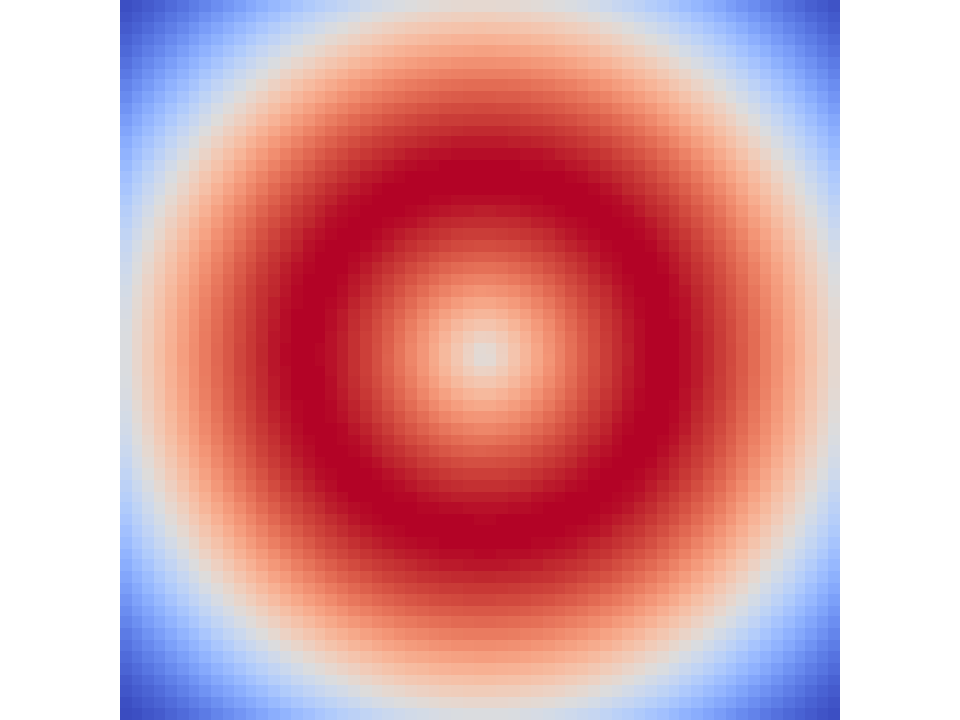
\includegraphics[scale=0.45]{figures/fgrid.pdf}
    % 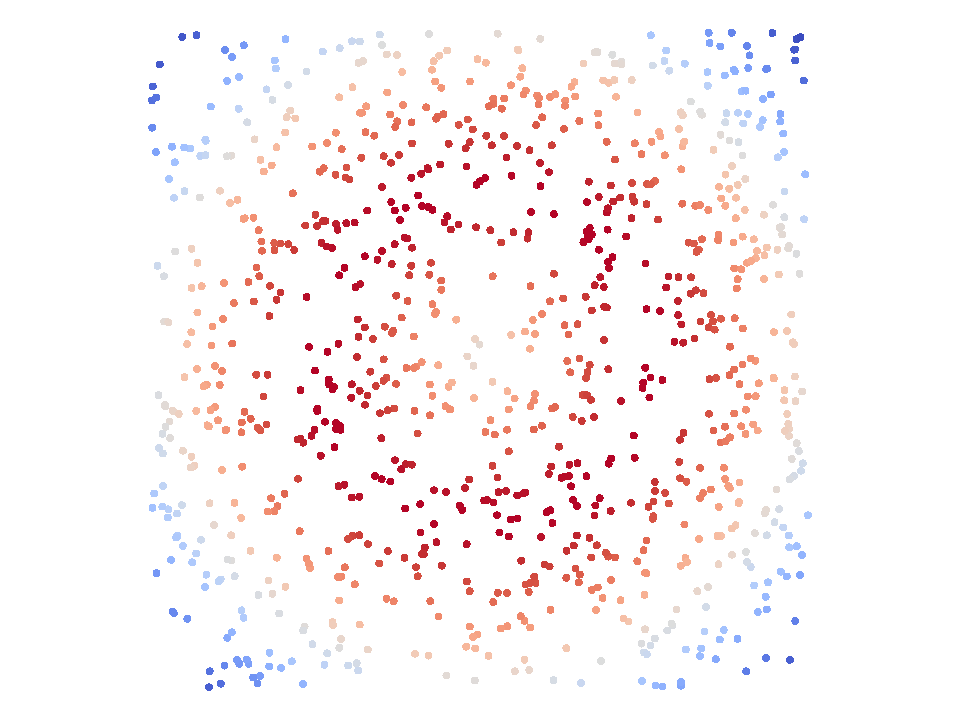
\includegraphics[scale=0.45]{figures/fsample.pdf}
    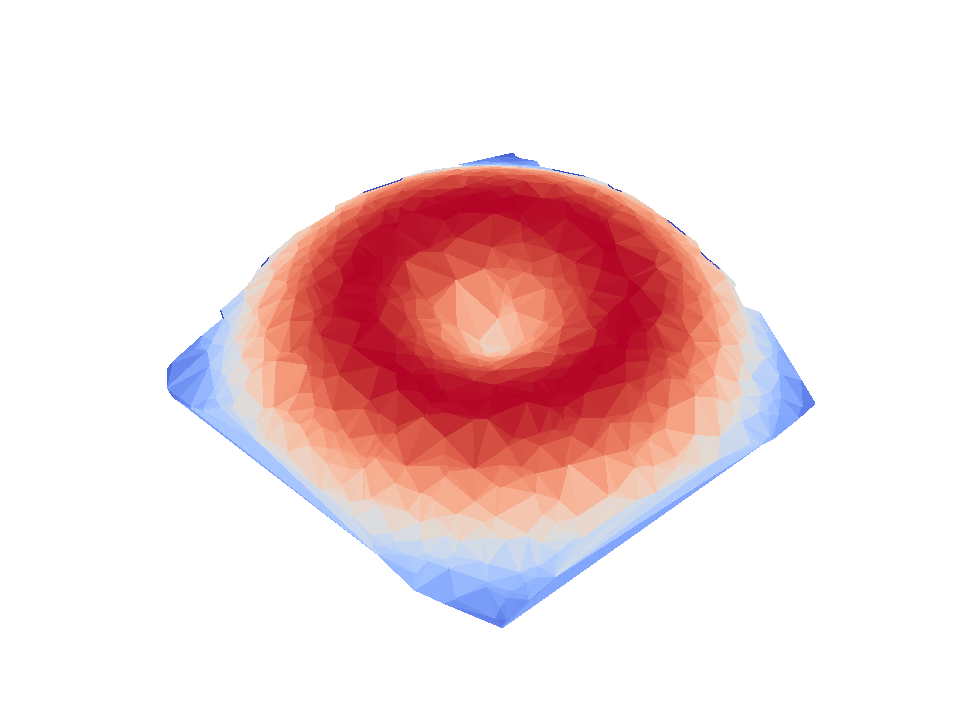
\includegraphics[scale=0.55]{figures/fcomplex.pdf}
    \caption{(Left) Continuous function on the plane.
            % (Middle) Function values on random sample.
            (Right) Function values on a random sample extended to a continuous piecewise linear approximation on a 2-dimension simplicial as the $z$-axis.}
    \label{fig:function}
\end{figure}}

Suppose we have some real valued function $f:\D\to\R$ and endow our sensors with the ability to measure this function at their points $P$.
If we know our network covers the domain we may construct a simplicial complex which captures its topology in a discrete structure.
We may therefore integrate the sparse measurements provided by the sensors throughout the simplicial complex to capture the topology of the function itself.
Not only do we now have a discrete approximation of the function but an ordering on the simplices of the complex which may be used to explore the evolution of the topological structure of the function.

This leads to a more general notion defined for a sequence of topological spaces, which we may take as sublevel sets of the function on the domain.
\begin{definition}
    Let $f:\D\to\R$ be a function on a topological domain $\D$ and let $I_0, I_1,\ldots$ be a sequence of intervals $I_i = [a_i, b_i)$ that covers the image of $f$ on $\D$.
    Let and $X_i = \{x\in\D\mid a_i\leq f(x) < b_i\}$ be topological subspaces connected by inclusion maps $X_i\to X_{i+1}$.
    A \textbf{filtration} is the resulting sequence of topological spaces
    \[X_0\to X_1\to\ldots X_i\to X_{i+1}\to\ldots .\]
\end{definition}
A filtration $\{K_i\}_{i=1,\ldots,n}$ may also be interpreted as a sequence of simplicial maps, each an inclusion $K_i\to K_{i+1}$.
This induces an algebraic sequence of homomorphisms on homology by functoriality, for all $k$:
\[ H_k(X_0)\to H_k(X_1)\to\ldots\to H_k(X_i)\to H_k(X_{i+1})\to\ldots . \]
This sequence encodes the local topological changes that occur at each step of the filtration.
Global information is encoded in terms of the \textbf{birth} and \textbf{death} of homology classes, represented as a \textbf{persistence diagram} or \textbf{barcode}.

% \vspace{0.25in}
% \textbf{TODO} Persistence diagram of a function on a simplicial complex
% \vspace{0.25in}

% \figblock{%
% \begin{figure}[htbp]
% \centering
%     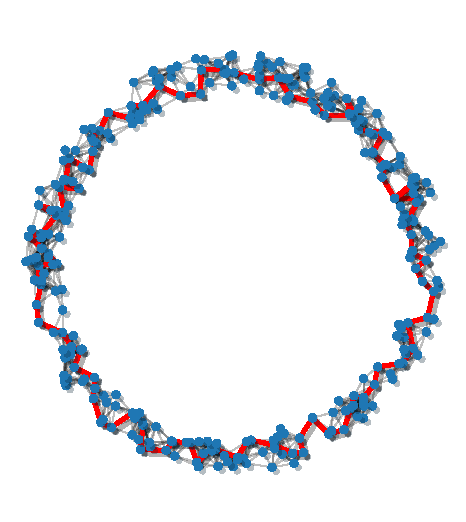
\includegraphics[scale=0.9]{figures/homology_cycle.pdf}\hspace{10ex}
%     % 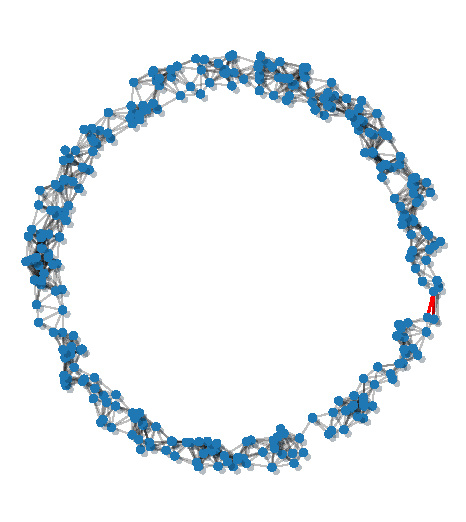
\includegraphics[scale=0.6]{figures/cohomology_cocycle.pdf}
%     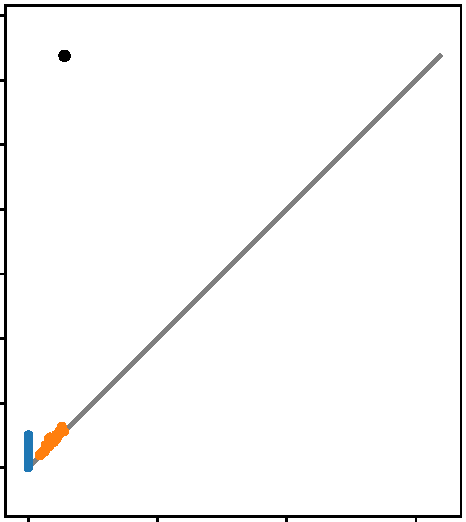
\includegraphics[scale=0.8]{figures/homology_dgm.pdf}
%     \caption{The representative cycle of a significant feature in the persistent homology of rips filtration of a noisy circle.
%             The birth of the feature indicated on the persistence diagram (right) corresponds to the scale of the rips complex shown (left) when the circle, a 1-cycle, is born.
%             The death of this feature corresponds to the scale of the rips complex at a larger scale (not shown) when a triangle first fills the interior of the circle.
%             This scale is approximately the length of the edges in the smallest equilateral triangle with sample points as vertices that contains the centroid of the sample.
%             This illustrates the geometric information encoded in the persistence diagram of geometric complexes as it is within a constant factor of the radius of the circle.}
%     \label{fig:cycle_diagrams}
% \end{figure}}
%
% Given a simplicial complex $K$ on a set of points $P\subset\D$ and a function $f:\D\to\R$ we may construct a filtration $\{K_i\}_{i=1,2,\ldots}$ by ordering the simplices by their function values.
% For example, $f(\sigma) = \max_{v\in\sigma} f(v)$ for any simplex $\sigma\in K$.
% The resulting filtration is now a sequence of simplicial maps, each an inclusion $K_i\to K_{i+1}$, which induces a sequence of homology groups.

% \subsection{Persistent Homology}
%
% \begin{figure}[htbp]
% \centering
%     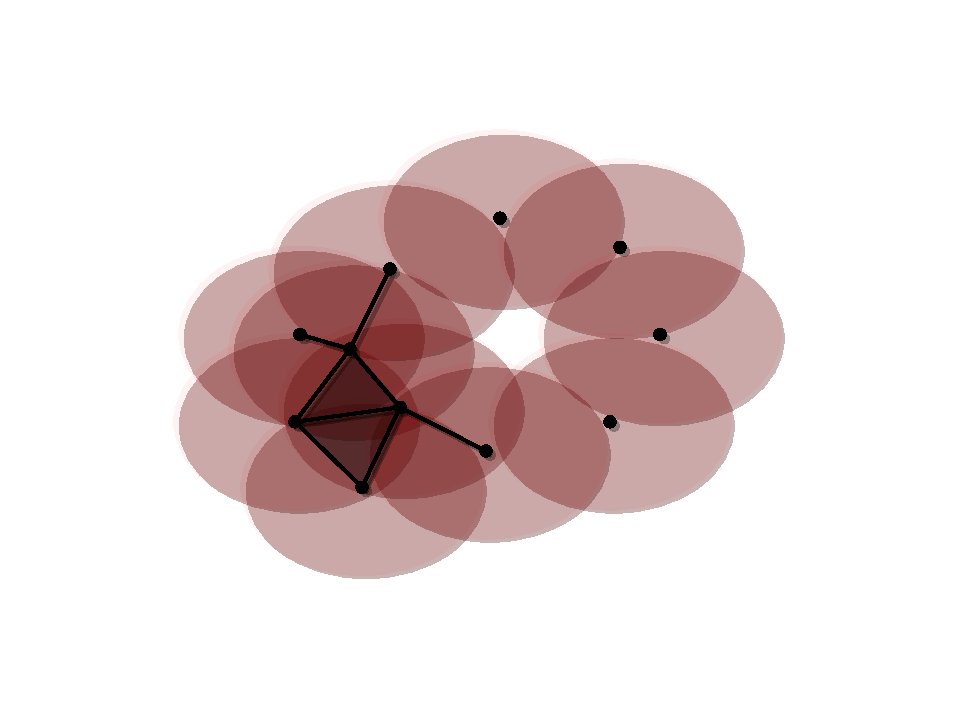
\includegraphics[scale=0.4]{figures/persist06.pdf}
%     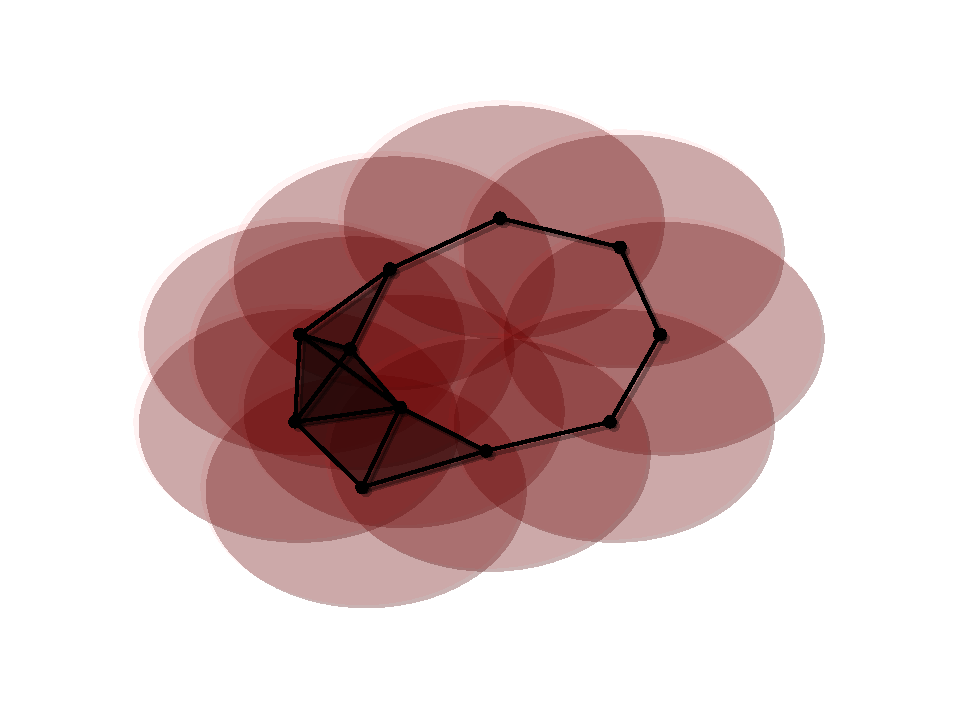
\includegraphics[scale=0.4]{figures/persist08.pdf}
%     % 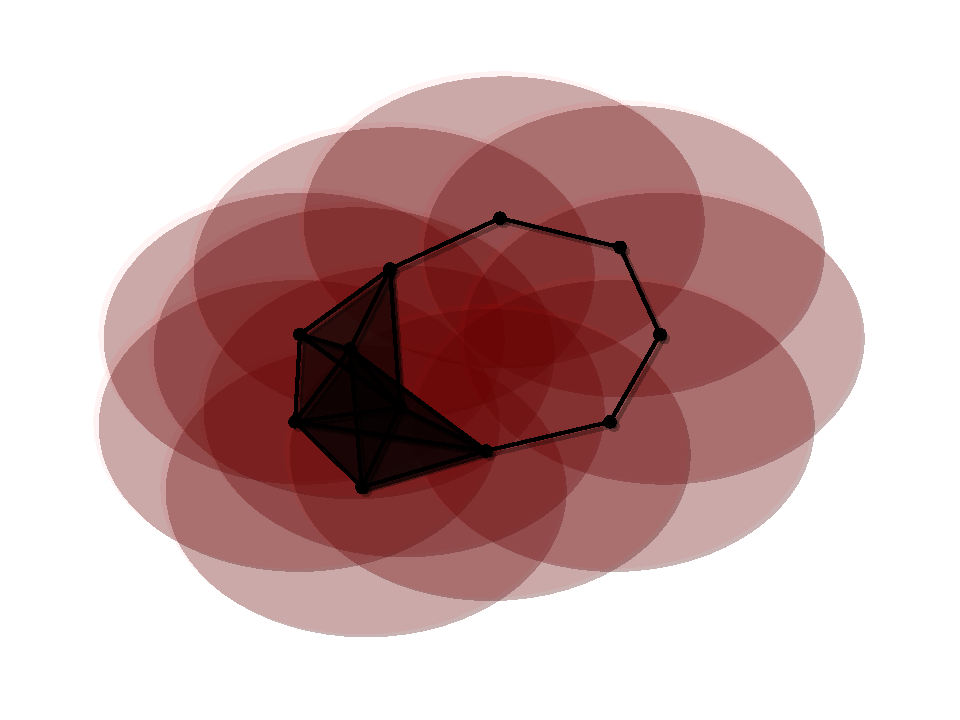
\includegraphics[scale=0.4]{figures/persist10.pdf}
%     % 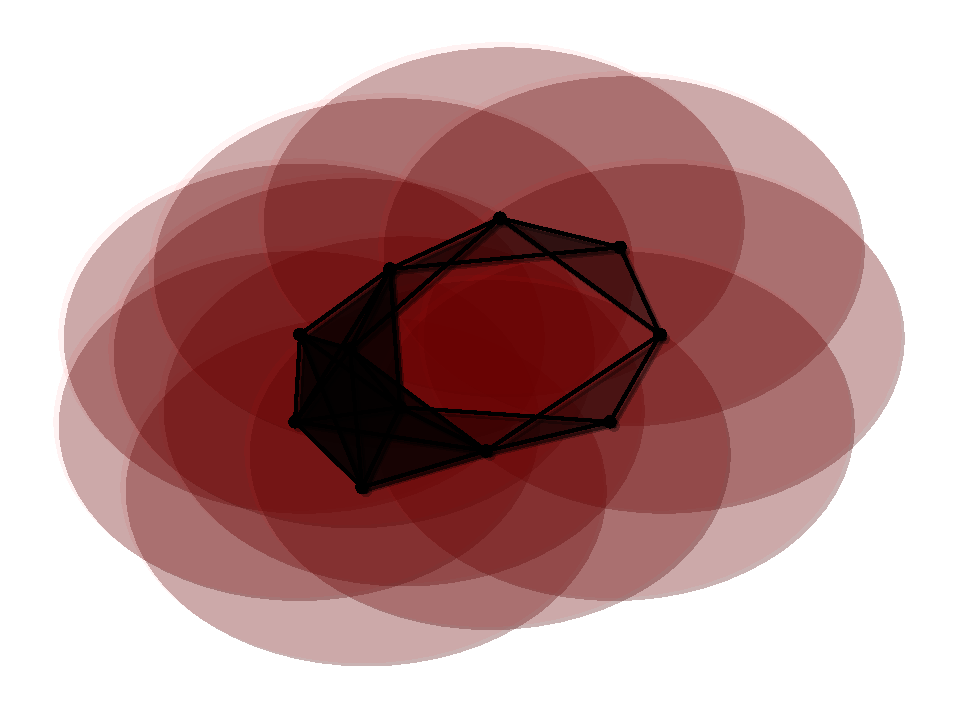
\includegraphics[scale=0.4]{figures/persist12.pdf}
%     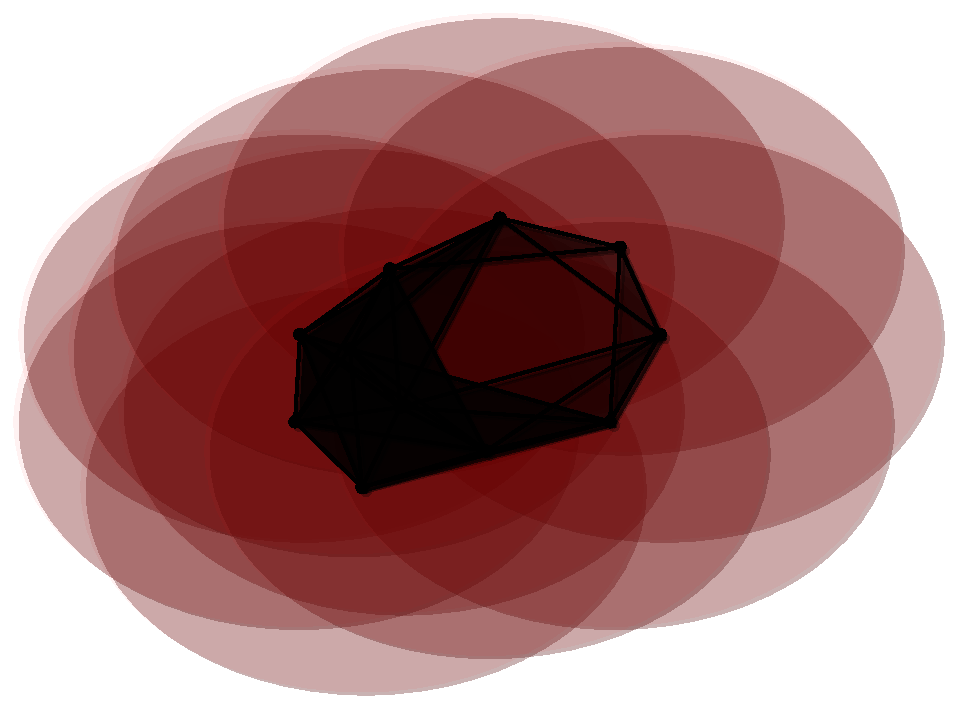
\includegraphics[scale=0.4]{figures/persist14.pdf}
%     \caption{A filtration of rips complexes at scales 0.6, 0.8, and 1.4 illustrating a point $(0.8, 1.4)$ in the corresponding persistence diagram. The 1-cycle that is born at scale 0.8 persists until it dies at scale 1.4.}
%     \label{fig:persist}
% \end{figure}
%
% % \vspace{0.25in}
% % \textbf{TODO} ``Metric'' persistence.
% % \vspace{0.25in}
%
% % Topological data analysis is an emerging field in the intersection of data analysis and algebraic topology which extends the notion of homology and cohomology groups to a more analytical tool known as \textbf{topological persistence}.
% % Where simplicial homology identifies invariants of a static simplicial complex persistent homology tracks the evolution of a sequence of nested simplicial complexes which provide a more detailed topological signature, in addition to relevant geometric information.
%
% Just as we can construct a filtration from a function on a simplicial complex we can construct a filtration from the metric induced on our sample by the domain.
% Let $P$ be a finite metric space with $m$ points and let $K = \rips_\alpha(P)$ be the Rips complex of $P$ at scale $\alpha$ consisting of $n$ simplices.
% We can order the simplices $\sigma_1,\ldots,\sigma_n$ by the minimum pairwise distance between their vertices by first applying an arbitrary ordering on the vertices $v_1,\ldots,v_m$ and letting $\sigma_i = \{v_i\}$ for $i=1,\ldots,m$ so that $K_i = \{\sigma_1,\ldots, \sigma_m\}$.
% We can then build a filtration $\K = \{K_i\}_{i=1,\ldots,n}$ so that $K_i = \rips_\e(P)$ where $\e = \max_{u,v\in\sigma_i}\dist(u,v)$ by adding one simplex at a time, breaking ties first by dimension, then by the ordering on their constituent vertices.
% A $k$-dimensional feature is identified when a $(k+1)$-simplex $\sigma$ is added that kills a $k$-cycle $\gamma$.
% In the persistence diagram, this feature would be represented by a point $(b, d)$ where $b$ is the smallest scale for which the $k$-cycle appears
% \[ \tau\in\rips_b(P)\text{ for all }\tau\in\gamma\]
% and $d = \max_{u,v\in\sigma}\dist(u,v)$ is the scale at which $\sigma$ enters the filtration.
% The result is a collection of points $(b_i, d_i)$ in the plane for each dimension $k$ known as the persistence diagram, denoted $\dgm_k(\K)$.
% A persistence diagram is depicted on the right in Fig.~\ref{fig:cycle_diagrams}.

\paragraph*{\textbf{Persistent Homology.}} % (fold)
\label{par:persistent_homology}

Given a filtration $\mathcal{F} = \{F_\alpha\}_{\alpha\in\R}$ the inclusions $F_\alpha\hookrightarrow F_\beta$ induce homeomorphisms between homology groups $h_*^{\alpha,\beta} : H_*(F_\alpha)\to H_*(F_\beta)$.
The \emph{persistent homology modules} of $\F$ are the pairs
\[\mathcal{H}_*(\F) = (\{H_*(F_\alpha)\}_{\alpha\in\R}, \{h_*^{\alpha,\beta}\}_{\alpha\leq\beta\in\R}).\]

The persistent homology modules of a filtration $\F$ are each given by a signature known as a \emph{persistence diagram}, denoted $\Pers_*(\F)$, where $\Pers(\F)$ is used to refer to the collection of persistence diagrams of all dimensions.
Unless otherwise noted we will refer $\Pers(\F)$ as the persistence diagram of $\F$.

The space of persistence diagrams is a metric space $(\PPers, \dist_B)$ under the \emph{bottleneck distance} which is defined for diagrams $A, B$, taken as multisets in $\R^2$ equipped with the $l^\infty$-norm, as
\[\dist_B(A, B) = \min_{\gamma:A\to B}\max_{p\in A} \| p- \gamma(p)\|_\infty\]
where $\gamma$ ranges over all bijections from $A$ to $B$.

\paragraph*{\textbf{Stability of Persistent Homology.}} % (fold)
\label{par:stability_of_persistent}

The persistent homology of Rips filtrations constructed from point clouds in euclidean space is closely related to the sequence of metric balls growing around the point cloud as the persistent homology of both gives a signature for distance to the point cloud.
In particular, the persistent homology of the Rips complex of a point cloud approximates that of the distance to the point cloud as a function on the underlying metric space.

\figblock{%
\begin{figure}[htbp]
\centering
    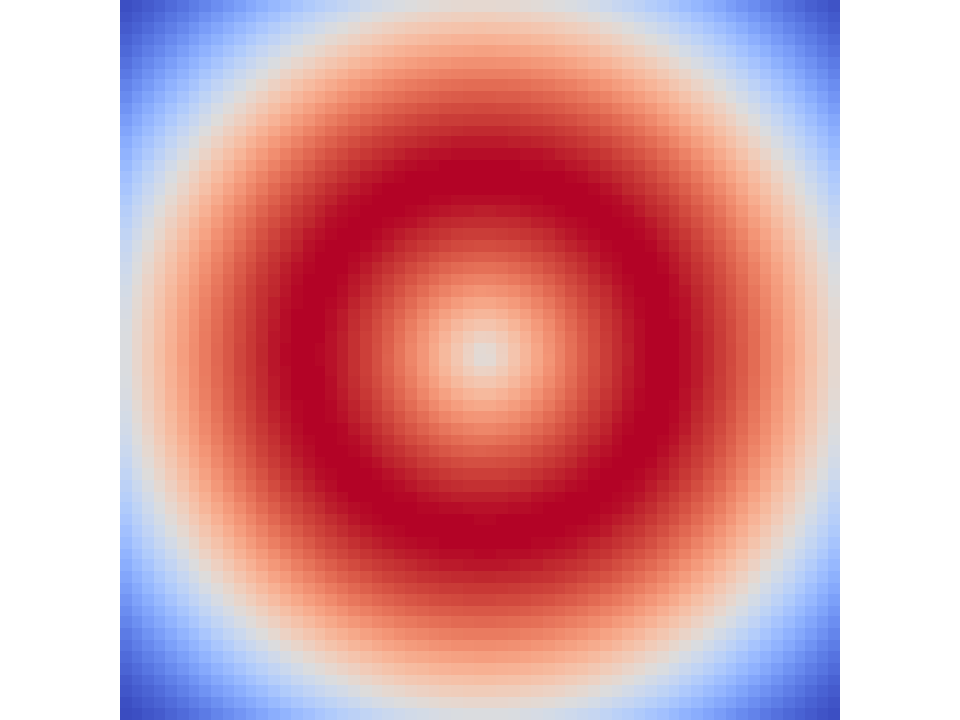
\includegraphics[width=0.29\textwidth,trim={0 -1.5cm 0 0},clip]{figures/fgrid.pdf}
    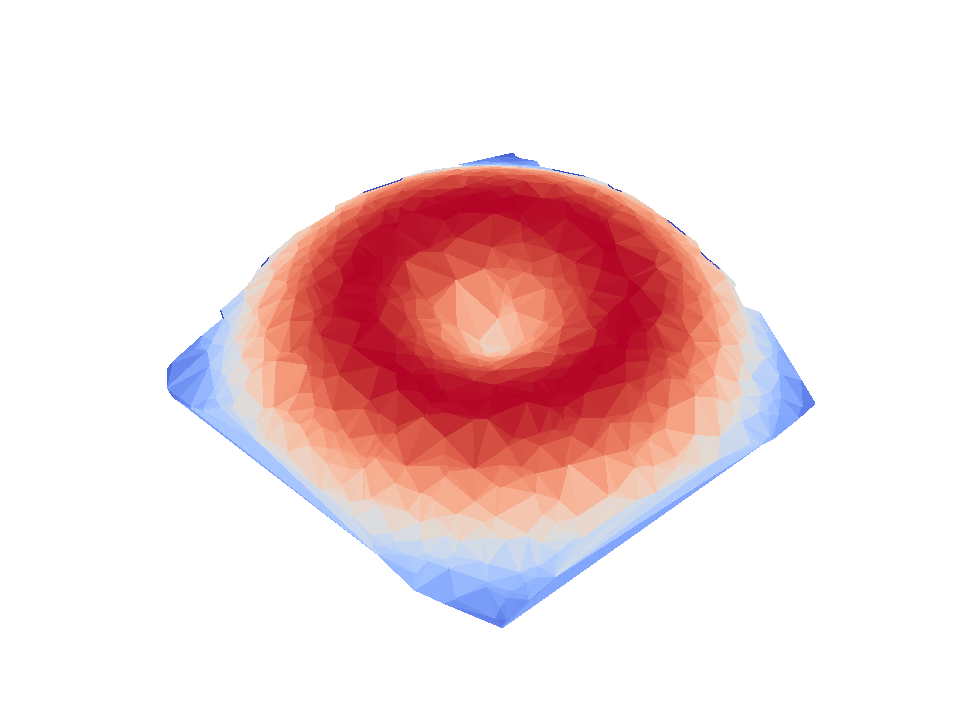
\includegraphics[width=0.4\textwidth]{figures/fcomplex.pdf}
    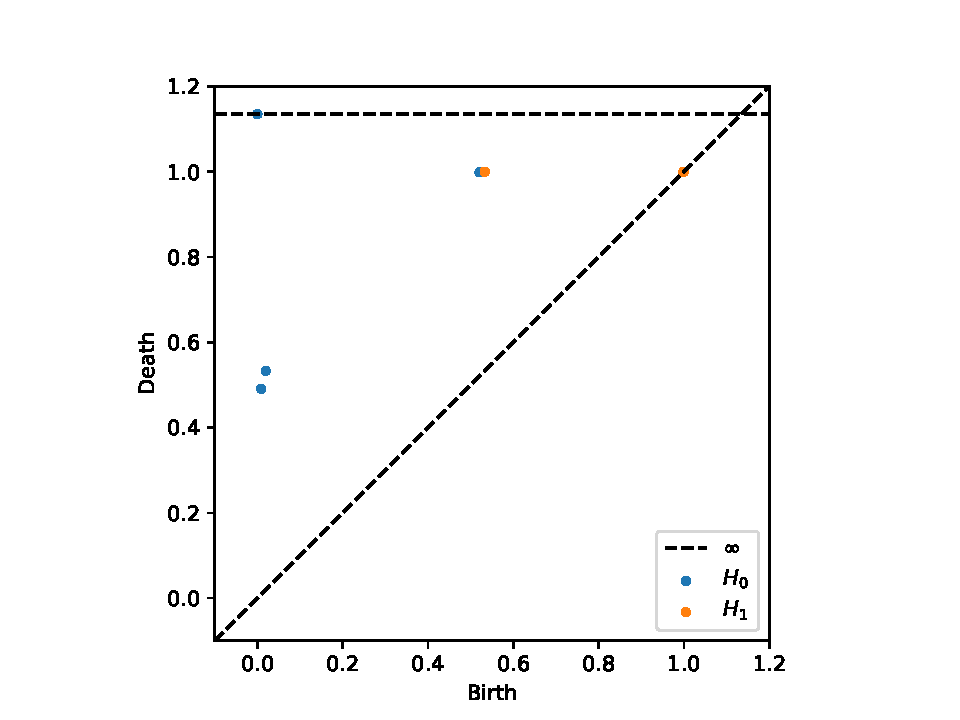
\includegraphics[width=0.29\textwidth,trim={2cm 0cm 2cm 1cm},clip]{figures/fdgm.pdf}
    \caption{(Left) Continuous function on the plane.
            (Middle) Function values (as $z$-axis) on a random sample extended to a simplicial complex.
            (Right) Persistence diagram of an induced filtration.}
    \label{fig:function}
\end{figure}
}

More generally, the persistent homology of a real-valued function captures the changes in the homology groups of its \emph{sublevel-sets}---the set of points with function values below a given scale.
The distance to a point cloud is a real-valued function with sublevel-sets equal to the union of metric balls at a given scale.
Under certain conditions we can approximate the persistent homology of a real-valued function given only its values on a finite subset of its domain.

Given a topological space $X$ and a real-valued function $f:X\to\R$ the \emph{sublevel-set filtration} of $f$ is the sequence $\{X^f_\alpha\}_{\alpha\in\R}$ of sublevel-sets $X^f_\alpha = f^{-1}(-\infty, \alpha]$.
We define a metric $\dmax$ between two real-valued functions $f,g:X\to\R$ by taking the maximum difference of the functions on any point, i.e.
\[ \dmax(f, g) := \max_{x\in X} |f(x) - g(x)|. \]

\begin{lemma}\label{lem:interleave}
    Let $X$ be a topological space and $f,g: X\to\R$ are tame functions such that $\dmax(f, g)\leq\e$.
    Then the sublevel-set filtrations $\{X_\alpha^f\}_{\alpha\in\R}$ of $f$ and $\{X_\alpha^g\}_{\alpha\in\R}$ of $g$ are $\e$-interleaved.
\end{lemma}

The following is a standard result in the stability of persistence diagrams.

\begin{lemma}\label{lem:stability}
    If two filtrations $\F$ and $\F'$ are $\e$-interleaved then
    \[ \dist_B(\Pers(\F), \Pers(\F'))\leq\e. \]
\end{lemma}

The persistent homology modules of the sublevel-set filtration $\{X^f_\alpha\}_{\alpha\in\R}$ are referred to as the persistent homology modules $\mathcal{H}_*(f)$ of $f$ with its diagram denoted $\Pers(f)$.

\begin{corollary}\label{cor:stability}
    If $X$ is a topological space and $f,g:X\to\R$ are tame functions then
    \[ \dist_B(\Pers(f), \Pers(g))\leq\dmax(f, g). \]
\end{corollary}
